\documentclass[journal,12pt,onecolumn]{IEEEtran}
\usepackage{graphicx, float}
\graphicspath{{Figs/}}
\usepackage{multicol}
\usepackage{parskip}
\usepackage{titlesec}
\usepackage{color}
\usepackage{enumitem}
\usepackage{amsmath,amssymb,amsfonts,amsthm}
\usepackage{array}
\usepackage{booktabs}
\usepackage[table]{xcolor}
\usepackage{longtable}
\usepackage{gensymb}
\usepackage{cite}
\usepackage{algorithmic}
\usepackage{textcomp}
\usepackage{txfonts}
\usepackage{listings}
\usepackage{mathtools}
\usepackage{comment}
\usepackage{tkz-euclide}
\usepackage[breaklinks=true]{hyperref}
\usepackage{gvv}
\usepackage[utf8]{inputenc}
\usetikzlibrary{arrows.meta, positioning}
\usepackage{xparse}
\usepackage{calc}
\usepackage{multirow}
\usepackage{hhline}
\usepackage{ifthen}
\usepackage{lscape}
\usepackage{tabularx}

\begin{document}

\title{
ASSIGNMENT 1: GATE 2023 \\
BT: BIOTECHNOLOGY ENGINEERING}
\author{AI25BTECH11025-R Nikhil}
\maketitle
\renewcommand{\thefigure}{\theenumi}
\renewcommand{\thetable}{\theenumi}


\title{GATE 2023 -- Biotechnology (BT)}
\date{}
\maketitle



\begin{enumerate}
    \item “You are delaying the completion of the task. Send ------------ contributions at the earliest.”
    \begin{enumerate}
        \item you are
        \item your
        \item you’re
        \item yore
    \end{enumerate}
    \hfill(GATE BT 2023)

    \item References : ------------ :: Guidelines : Implement (By word meaning)
    \begin{enumerate}
        \item Sight
        \item Site
        \item Cite
        \item Plagiarise
    \end{enumerate}
    \hfill(GATE BT 2023)

    \item In the given figure, PQRS is a parallelogram with PS = 7 cm, PT = 4 cm and PV = 5 cm. What is the length of RS in cm? (The diagram is representative.)
    \begin{figure}[H]
        \centering
        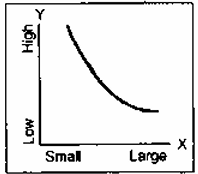
\includegraphics[width=0.8\textwidth]{Fig 1.png}
        \caption{}
        \label{fig:question3}
    \end{figure}
    \begin{enumerate}
        \item $\frac{20}{7}$
        \item $\frac{28}{5}$
        \item $\frac{9}{2}$
        \item $\frac{35}{4}$
    \end{enumerate}
    \hfill(GATE BT 2023)

    \item In 2022, June Huh was awarded the Fields medal, which is the highest prize in Mathematics. When he was younger, he was also a poet. He did not win any medals in the International Mathematics Olympiads. He dropped out of college. Based only on the above information, which one of the following statements can be logically inferred with certainty?
    \begin{enumerate}
        \item Every Fields medalist has won a medal in an International Mathematics Olympiad.
        \item Everyone who has dropped out of college has won the Fields medal.
        \item All Fields medalists are part-time poets.
        \item Some Fields medalists have dropped out of college.
    \end{enumerate}
    \hfill(GATE BT 2023)

    \item A line of symmetry is defined as a line that divides a figure into two parts in a way such that each part is a mirror image of the other part about that line. The given figure consists of 16 unit squares arranged as shown. In addition to the three black squares, what is the minimum number of squares that must be coloured black, such that both PQ and MN form lines of symmetry? (The figure is representative)
    \begin{figure}[H]
        \centering
        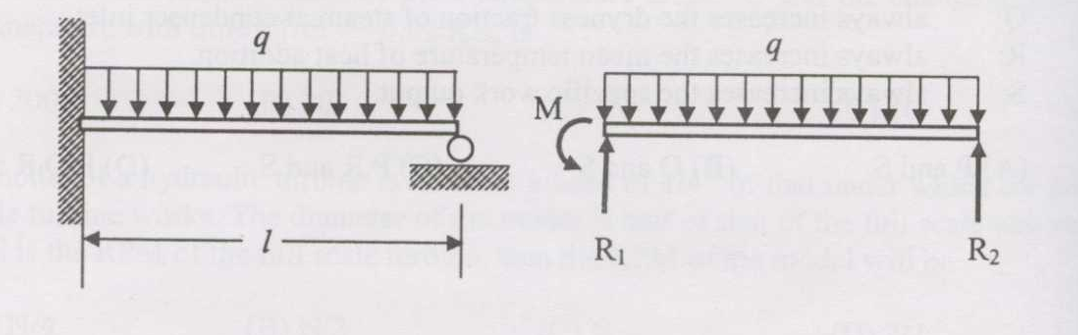
\includegraphics[width=0.8\textwidth]{Fig 2.png}
        \caption{}
        \label{fig:question5}
    \end{figure}
    \begin{enumerate}
        \item 3
        \item 4
        \item 5
        \item 6
    \end{enumerate}
    \hfill(GATE BT 2023)

    \item Human beings are one among many creatures that inhabit an imagined world. In this imagined world, some creatures are cruel. If in this imagined world, it is given that the statement “Some human beings are not cruel creatures” is FALSE, then which of the following set of statement(s) can be logically inferred with certainty?
    \begin{enumerate}
        \item[(i)] All human beings are cruel creatures.
        \item[(ii)] Some human beings are cruel creatures.
        \item[(iii)] Some creatures that are cruel are human beings.
        \item[(iv)] No human beings are cruel creatures.
    \end{enumerate}
    \begin{enumerate}
        \item only (i)
        \item only (iii) and (iv)
        \item only (i) and (ii)
        \item (i), (ii) and (iii)
    \end{enumerate}
    \hfill(GATE BT 2023)

    \item To construct a wall, sand and cement are mixed in the ratio of 3:1. The cost of sand and that of cement are in the ratio of 1:2. If the total cost of sand and cement to construct the wall is 1000 rupees, then what is the cost (in rupees) of cement used?
    \begin{enumerate}
        \item 400
        \item 600
        \item 800
        \item 200
    \end{enumerate}
    \hfill(GATE BT 2023)

    \item The World Bank has declared that it does not plan to offer new financing to Sri Lanka, which is battling its worst economic crisis in decades, until the country has an adequate macroeconomic policy framework in place. In a statement, the World Bank said Sri Lanka needed to adopt structural reforms that focus on economic stabilisation and tackle the root causes of its crisis. The latter has starved it of foreign exchange and led to shortages of food, fuel, and medicines. The bank is repurposing resources under existing loans to help alleviate shortages of essential items such as medicine, cooking gas, fertiliser, meals for children, and cash for vulnerable households. Based only on the above passage, which one of the following statements can be inferred with certainty?
    \begin{enumerate}
        \item According to the World Bank, the root cause of Sri Lanka’s economic crisis is that it does not have enough foreign exchange.
        \item The World Bank has stated that it will advise the Sri Lankan government about how to tackle the root causes of its economic crisis.
        \item According to the World Bank, Sri Lanka does not yet have an adequate macroeconomic policy framework.
        \item The World Bank has stated that it will provide Sri Lanka with additional funds for essentials such as food, fuel, and medicines.
    \end{enumerate}
    \hfill(GATE BT 2023)

    \item The coefficient of $x^4$ in the polynomial $(x - 1)^3(x - 2)^3$ is equal to ------------.
    \begin{enumerate}
        \item 33
        \item $-3$
        \item 30
        \item 21
    \end{enumerate}
    \hfill(GATE BT 2023)

    \item Which one of the following shapes can be used to tile (completely cover by repeating) a flat plane, extending to infinity in all directions, without leaving any empty spaces in between them? The copies of the shape used to tile are identical and are not allowed to overlap.
    \begin{enumerate}
        \item circle
        \item regular octagon
        \item regular pentagon
        \item rhombus
    \end{enumerate}
    \hfill(GATE BT 2023)

    \item Eukaryotic transcription is carried out by
    \begin{enumerate}
        \item DNA-dependent RNA polymerase
        \item DNA-dependent DNA polymerase
        \item RNA-dependent DNA polymerase
        \item RNA-dependent RNA polymerase
    \end{enumerate}
    \hfill(GATE BT 2023)

    \item Acetylcholine released by the parasympathetic nerves has which one of the following functions in the heart pacemaker cells?
    \begin{enumerate}
        \item It binds to GPCR and activates G protein to slow the heart rate
        \item It stimulates GABA-activated ion-channel coupled receptor to increase the heart rate
        \item It binds to GPCR and inhibits G protein to slow the heart rate
        \item It inhibits GABA-activated ion-channel coupled receptor to increase the heart rate
    \end{enumerate}
    \hfill(GATE BT 2023)

    \item Determine the correctness or otherwise of the following Assertion [a] and the Reason [r].
    
    Assertion [a]: In multicellular organisms, cells of different lineages have different gene expression profiles.
    
    Reason [r]: Alternative splicing is the only mechanism to generate protein diversity.
    \begin{enumerate}
        \item Both [a] and [r] are false
        \item Both [a] and [r] are true and [r] is the correct reason for [a]
        \item Both [a] and [r] are true but [r] is not the correct reason for [a]
        \item [a] is true but [r] is false
    \end{enumerate}
    \hfill(GATE BT 2023)

    \item Determine the correctness or otherwise of the following Assertion [a] and the Reason [r].
    
    Assertion [a]: Chromosome mutations can change the structure of chromosomes.
    
    Reason [r]: All chromosome mutations arise due to nondisjunction of chromosomes during mitosis or meiosis.
    \begin{enumerate}
        \item Both [a] and [r] are false
        \item [a] is true but [r] is false
        \item Both [a] and [r] are true and [r] is the correct reason for [a]
        \item Both [a] and [r] are true but [r] is not the correct reason for [a]
    \end{enumerate}
    \hfill(GATE BT 2023)

    \item C-value paradox refers to
    \begin{enumerate}
        \item the lack of correlation between genome size and genetic complexity of an organism
        \item the presence of genetic sequences that propagate themselves within a genome
        \item the coexistence of multiple alleles at a genetic locus
        \item the concept that two or more genes may have the same function
    \end{enumerate}
    \hfill(GATE BT 2023)

    \item Which one of the following drugs is NOT an immune checkpoint inhibitor?
    \begin{enumerate}
        \item Ipilimumab
        \item Pembrolizumab
        \item Nivolumab
        \item Trastuzumab
    \end{enumerate}
    \hfill(GATE BT 2023)

    \item Dendritic cells are involved in cross-presentation of antigens. Which of the following protein(s) is(are) required for cross-presentation? 
    \begin{enumerate}
        \item[P.] Basic leucine zipper ATF-like transcription factor 3 (BATF3)
        \item[Q.] Membrane associated ring-CH-type finger 1 (MARCH-1)
        \item[R.] Solute carrier family 10 member 1 (SLC10A1)
        \item[S.] Class II-associated invariant chain peptide (CLIP)
    \end{enumerate}
    \begin{enumerate}
        \item P only
        \item P and R only
        \item P, Q and R only
        \item S only
    \end{enumerate}
    \hfill(GATE BT 2023)

    \item Which one of the following is required for the development of B-cells in the bone marrow?
    \begin{enumerate}
        \item Stromal cells
        \item Dendritic cells
        \item Kupffer cells
        \item NK cells
    \end{enumerate}
    \hfill(GATE BT 2023)

    \item Which one of the following statements is TRUE about leghemoglobin?
    \begin{enumerate}
        \item It binds oxygen to protect nitrogenase
        \item It binds hemoglobin to protect oxygenase
        \item It binds oxygen to protect hydrogenase
        \item It binds oxygen to protect oxygenase
    \end{enumerate}
    \hfill(GATE BT 2023)

    \item The correct sequence of events during bacteriophage infection of a bacterial cell is
    \begin{enumerate}
        \item landing $\rightarrow$ attachment $\rightarrow$ tail contraction $\rightarrow$ penetration and unplugging $\rightarrow$ DNA ejection
        \item attachment $\rightarrow$ landing $\rightarrow$ penetration and unplugging $\rightarrow$ tail contraction $\rightarrow$ DNA ejection
        \item landing $\rightarrow$ tail contraction $\rightarrow$ attachment $\rightarrow$ DNA ejection $\rightarrow$ penetration and unplugging
        \item attachment $\rightarrow$ tail contraction $\rightarrow$ landing $\rightarrow$ penetration and unplugging $\rightarrow$ DNA ejection
    \end{enumerate}
    \hfill(GATE BT 2023)

    \item Intracellular proteins are targeted for proteolytic degradation in proteasomes upon conjugation with
    \begin{enumerate}
        \item ubiquitin
        \item integrin
        \item peptidase
        \item calreticulin
    \end{enumerate}
    \hfill(GATE BT 2023)

    \item In ELISA, which of the following enzymes are conjugated to antibodies for detection of the analyte?
    \begin{enumerate}
        \item[P.] Alkaline phosphatase
        \item[Q.] Trypsinase
        \item[R.] Horseradish peroxidase
        \item[S.] Amylase
    \end{enumerate}\hfill(GATE BT 2023)
    \begin{enumerate}
        \item P and R
        \item P and Q
        \item Q and S
        \item R and S
    \end{enumerate}
    \hfill(GATE BT 2023)

    \item In hybridoma technology, which one of the following enzymes is absent in the myeloma cells that are used for monoclonal antibody production?
    \begin{enumerate}
        \item Hypoxanthine-guanine phosphoribosyltransferase
        \item Alanine aminotransferase
        \item Triose phosphate isomerase
        \item Glycosyltransferase
    \end{enumerate}
    \hfill(GATE BT 2023)

    \item Which of the following methods are used for detection of DNA and RNA, respectively?
    \begin{enumerate}
        \item Southern and Northern blotting
        \item Southern and Western blotting
        \item Northern and Southern blotting
        \item Northern and Western blotting
    \end{enumerate}
    \hfill(GATE BT 2023)

    \item Match the types of RNA in Group I with their functions in Group II.
    \begin{table}[H]
    \begin{tabular}{ll}
    
        Group I & Group II \\
        P. mRNA & 1. Serves as adaptors between mRNA and amino acids during protein synthesis \\
        Q. rRNA & 2. Regulates post-transcriptional gene expression \\
        R. miRNA & 3. Codes for proteins \\
        S. tRNA & 4. Forms the core of the ribosome structure and catalyzes protein synthesis \\
     \end{tabular}
     \caption{}
     \label{match the following}
    \end{table}
    
    
    \begin{enumerate}
        \item P-3, Q-4, R-2, S-1
        \item P-3, Q-4, R-1, S-2
        \item P-4, Q-3, R-2, S-1
        \item P-2, Q-1, R-4, S-3
    \end{enumerate}
    \hfill(GATE BT 2023)

    \item Which one of the following programs is used for finding distantly related (or remote) protein homologs?
    \begin{enumerate}
        \item BLASTN
        \item BLASTX
        \item PSI-BLAST
        \item TBLASTX
    \end{enumerate}
    \hfill(GATE BT 2023)

    \item Which one of the following is used for global alignment of two protein sequences?
    \begin{enumerate}
        \item Chou-Fasman method
        \item Garnier-Osguthorpe-Robson (GOR) method
        \item Needleman-Wunsch algorithm
        \item Smith-Waterman algorithm
    \end{enumerate}
    \hfill(GATE BT 2023)

    \item Which one of the following methods CANNOT be used to determine the secondary structure content of a protein?
    \begin{enumerate}
        \item Circular dichroism spectroscopy
        \item Fourier transform infrared spectroscopy
        \item Mass spectrometry
        \item X-ray crystallography
    \end{enumerate}
    \hfill(GATE BT 2023)

    \item Which one of the following plant growth regulators facilitate adventitious root formation?
    \begin{enumerate}
        \item Auxin
        \item Zeatin
        \item Dihydrozeatin
        \item Kinetin
    \end{enumerate}
    \hfill(GATE BT 2023)

    \item Fabry disease in humans is a X-linked disease. The probability (in percentage) for a phenotypically normal father and a carrier mother to have a son with Fabry disease is ------------.

\hfill(GATE BT 2023)

    \item The value of $\lim_{x \to 0} \left[ \frac{\cos 2x - \cos 4x}{x^2} \right]$ is ------------.

    \item A series (S) is given as
    
    S = 1 + 3 + 5 + 7 + 9 + ……
    
    The sum of the first 50 terms of S is ------------.

    \hfill(GATE BT 2023)

    \item Two fair six-sided dice are thrown. The probability of getting 12 as the product of the numbers on the dice (rounded off to two decimal places) is ------------.

    \hfill(GATE BT 2023)

    \item If $7^{3x} = 216$, the value of $7^{-x}$ (rounded off to three decimal places) is ------------.

    \hfill(GATE BT 2023)

    \item The distance between the two points of intersection of $x^2 + y = 7$ and $x + y = 7$ (rounded off to two decimal places) is ------------.

    \hfill(GATE BT 2023)

    \item Match the immunological terms in Group I with their descriptions in Group II.
    
    \begin{tabular}{ll}
        Group I & Group II \\
        P. Anergy & 1. Elimination of activated T-cells after antigen clearance \\
        Q. Activation-induced cell death & 2. Inhibition of auto-reactive T-cells at periphery \\
        R. Receptor editing & 3. Unresponsiveness to antigens due to lack of co-stimulatory molecules \\
        S. Regulatory T-cells & 4. Elimination of auto-reactive B-cells \\
    \end{tabular}
    
    \begin{enumerate}
        \item P-3, Q-1, R-4, S-2
        \item P-4, Q-3, R-1, S-2
        \item P-3, Q-4, R-2, S-1
        \item P-3, Q-2, R-4, S-1
    \end{enumerate}
    \hfill(GATE BT 2023)

    \item Match the type of bacteria in Group I with their respective growth properties in Group II.
    
    \begin{tabular}{ll}
        Group I & Group II \\
        P. Halophile & 1. Grows optimally between 20 $^\circ$C and 45 $^\circ$C \\
        Q. Piezophile & 2. Grows best at low water activity \\
        R. Mesophile & 3. Grows at high level of salt \\
        S. Xerophile & 4. Grows optimally at high hydrostatic pressure \\
    \end{tabular}
    
    \begin{enumerate}
        \item P-3, Q-4, R-1, S-2
        \item P-2, Q-3, R-4, S-1
        \item P-3, Q-1, R-2, S-4
        \item P-4, Q-3, R-1, S-2
    \end{enumerate}
    \hfill(GATE BT 2023)

    \item Match the viruses in Group I with their genome types in Group II.
    
    \begin{tabular}{ll}
        Group I & Group II \\
        P. T4 bacteriophage & 1. dsRNA \\
        Q. SARS-CoV-2 & 2. ssDNA \\
        R. Pseudomonas phage $\phi$6 & 3. dsDNA \\
        S. $\phi$X174 bacteriophage & 4. ssRNA \\
    \end{tabular}
    
    \begin{enumerate}
        \item P-3, Q-4, R-1, S-2
        \item P-2, Q-1, R-4, S-3
        \item P-4, Q-3, R-2, S-1
        \item P-1, Q-4, R-2, S-3
    \end{enumerate}
    \hfill(GATE BT 2023)

    \item The event(s) that lead(s) to inactivation of tumor suppressor genes in cancer cells is(are)
    \begin{enumerate}
        \item gene amplification
        \item promoter methylation
        \item loss of heterozygosity
        \item histone acetylation
    \end{enumerate}
    \hfill(GATE BT 2023)

    \item Methylation of CpG islands near the promoter of a gene can inhibit transcription by
    \begin{enumerate}
        \item preventing RNA polymerase binding
        \item facilitating repressor binding
        \item facilitating heterochromatin formation
        \item inducing euchromatin formation
    \end{enumerate}
    \hfill(GATE BT 2023)

    \item Which of the following statement(s) is(are) TRUE about induced pluripotent stem cells?
    \begin{enumerate}
        \item They can self-renew
        \item They require specific signals to maintain their stemness
        \item They cannot be genetically manipulated
        \item They can form organoids in vitro
    \end{enumerate}
    \hfill(GATE BT 2023)

    \item Which of the following statement(s) is(are) TRUE about fluoroquinolone drugs?
    \begin{enumerate}
        \item They contain quinolone ring(s)
        \item They inhibit RNA polymerase
        \item They bind to bacterial topoisomerase
        \item They bind to 23S rRNA within the 50S ribosome subunit
    \end{enumerate}
    \hfill(GATE BT 2023)

    \item Which of the following is(are) plant protoplast fusogenic agent(s)?
    \begin{enumerate}
        \item Sodium nitrate
        \item Polyvinyl alcohol
        \item Polyethylene glycol
        \item Bromoxynil
    \end{enumerate}
    \hfill(GATE BT 2023)

    \item Direct DNA transfer method(s) used for plant genetic engineering is(are)
    \begin{enumerate}
        \item microparticle bombardment
        \item electroporation
        \item polyethylene glycol treatment
        \item Agrobacterium-mediated transformation
    \end{enumerate}
    
    \hfill(GATE BT 2023)

    \item Which of the following vector(s) is(are) used to clone a DNA fragment of size 220 kb?
    \begin{enumerate}
        \item Bacterial artificial chromosome
        \item Yeast artificial chromosome
        \item Cosmids
        \item pUC19 plasmid
    \end{enumerate}\hfill(GATE BT 2023)

    \item The following reaction represents biomass synthesis from hexadecane 
    
    $C_{16}H_{34} + 12.5O_2 + 2.13NH_3 \rightarrow 10.6CH_{1.66}O_{0.27}N_{0.27} + 5.37CO_2 + 11.4H_2O$
    
    where $CH_{1.66}O_{0.27}N_{0.27}$ represents the biomass. The value of respiratory quotient (rounded off to two decimal places) is ------------.

    \hfill(GATE BT 2023)

    \item Temperature of a reaction with an activation energy value of $15 \text{ kcal.mol}^{-1}$ is increased from 300 K to 310 K. If the value of the ideal gas constant (R) is $1.9872 \text{ cal.mol}^{-1}.\text{K}^{-1}$, the ratio of the reaction rate constants $(k_{310}/k_{300})$ (rounded off to two decimal places) is ------------.

    \hfill(GATE BT 2023)

    \item E. coli is cultivated in a chemostat operated at a dilution rate of $0.2 \text{ h}^{-1}$. The values of biomass yield due to oxygen consumption and the steady state biomass concentration are $0.2 \text{ g.g}^{-1}$ and $10 \text{ g.L}^{-1}$, respectively. The oxygen transfer rate (in $\text{g.L}^{-1}\text{h}^{-1}$) is ------------.

    \hfill(GATE BT 2023)

    \item Aqueous two-phase extraction is used to recover $\alpha$-amylase from a solution. A polypropylene glycol-dextran mixture is added and the solution separates into upper and lower phases. The partition coefficient is 4.0 and the ratio of upper to lower phase volume is 5.0. The enzyme recovery or yield (in percentage, rounded off to the nearest integer) is ------------.

    \hfill(GATE BT 2023)

    \item E. coli cultivated at 298 K uptakes an uncharged compound (A) by passive diffusion. The intracellular and extracellular concentrations of A are 0.001 M and 0.1 M, respectively. If the value of the ideal gas constant R is $1.9872 \text{ cal.mol}^{-1}.\text{K}^{-1}$, the free-energy change (in $\text{kcal.mol}^{-1}$) for this passive diffusion of A (rounded off to two decimal places) is ------------.

    \hfill(GATE BT 2023)

    \item If there are three unrooted trees for four protein sequences, the number of rooted trees for the same number of sequences is ------------.

    \hfill(GATE BT 2023)

    \item The number of different possible ways of forming five intramolecular disulfide bonds with ten cysteine residues of a protein is ------------.

    \hfill(GATE BT 2023)

    \item The following schematic diagram shows a chemostat with cell recycle
    \begin{figure}[H]
        \centering
        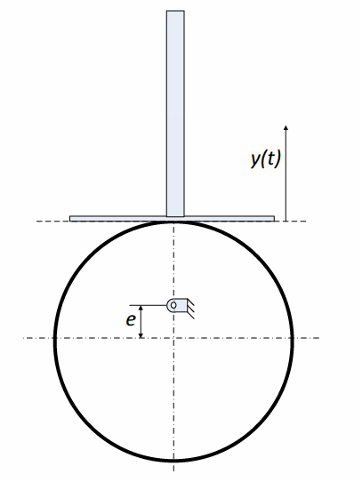
\includegraphics[width=0.8\textwidth]{Fig 3.png}
        \caption{}
        \label{fig:question53}
    \end{figure}
    where $F_0$ and $F_r$ are the volumetric flow rates (in L.h$^{-1}$) of feed and recycle streams, respectively. $X_1$, $X_0$ and $X$ are the cell concentrations (in g.L$^{-1}$) in the reactor, recycle-stream and product-stream, respectively. If $\frac{X_0}{X_1} = 1.5$, $\frac{F_r}{F_0} = 0.7$ and $X_1$ is $7.3 \text{ g.L}^{-1}$, the value of $X$ (in g.L$^{-1}$, rounded off to one decimal place) is ------------.

    \hfill(GATE BT 2023)

    \item An enzyme (E) catalyzes the biochemical reaction A $\rightarrow$ B with $k_{cat}$ equal to $500 \text{ s}^{-1}$. If the initial reaction velocity ($V_0$) is $10 \mu\text{M.s}^{-1}$ at the total enzyme concentration $[E_t]$ of 30 nM and substrate concentration [A] of $40 \mu\text{M}$, the value of $K_m$ (in $\mu\text{M}$) is ------------.

    \hfill(GATE BT 2023)

    \item DNA sample collected from an unidentified bacterial species (Y) contains 13\% of adenine. The G+C content (in percentage) of Y is ------------.

    \hfill(GATE BT 2023)

    \item If 1000 bp of a double-helical DNA weighs $1 \times 10^{-18}$ gm and distance between two bp is 0.34 nm, the total amount of DNA (in mg, rounded off to one decimal place) required to stretch from Earth to Moon (assuming the distance between Earth and Moon to be 3,74,000 km) is ------------.

    \hfill(GATE BT 2023)

    \item A protein has three identical sites arranged at the vertices of an equilateral triangle. If one site is filled with a dye (donor), the measured quantum yield ($\phi_D$) is 0.5. Filling one site with a donor dye and a second site with an acceptor dye results in $\phi_D$ of 0.25. The measured $\phi_D$ of one site filled with donor and the other two sites filled with acceptor dye (rounded off to three decimal places) is ------------.

    \hfill(GATE BT 2023)

    \item If $A = \begin{pmatrix} 1 & 2 \\ 3 & 5 \end{pmatrix}$, the value of $|A^4 + 3A^2 - 5A + 6I|$ is ------------.

    \hfill(GATE BT 2023)

    \item If $f(x) = \frac{\sin x + \cos x}{\sin x - \cos x}$, the value of $f'(x)$ at $x = 0$ is ------------.

    \hfill(GATE BT 2023)

    \item If $f(2) = 5$ and $(f(x))(f(x+1)) = 3$ for all real values of $x$, the value of $f(10)$ is ------------.

    \hfill(GATE BT 2023)

    \item Ten playing cards numbered 1, 2, 3, ..., 10 are placed face down on a table. One card is drawn at random, its number recorded, and then replaced face down. A card is drawn again at random. The probability that the number on the second draw is greater than the number on the first draw (rounded off to two decimal places) is ------------.

    \hfill(GATE BT 2023)

    \item The values of the consistency index ‘K’ and the flow behavior index ‘n’ of a dilatant fluid are 0.415 (in CGS units) and 1.23, respectively. The value of the apparent viscosity (in g.cm$^{-1}$.s$^{-1}$) of this fluid at a shear rate of 60 s$^{-1}$ (rounded off to the nearest integer) is ------------.

    \hfill(GATE BT 2023)

    \item An evaporator is insulated using glass wool material of 0.15 m thickness. The inner most surface and the outer surface of the insulation are at 700 $^\circ$C and 80 $^\circ$C, respectively. The mean thermal conductivity of the glass wool under these conditions is 0.29 W.m$^{-1}$.K$^{-1}$. The rate of heat loss (in W) through 1.2 m$^2$ of the evaporator wall surface (rounded off to the nearest integer) is ------------.

    \hfill(GATE BT 2023)

    \item A proportional controller is used to control the temperature of an autoclave from 60$^\circ$C to 130$^\circ$C. If the proportional band setting of the controller is 25\%, the proportional gain value is ------------.

    

    \item A dNTP master-mix is prepared by combining 40 $\mu$L of each 20 mM dNTP stock (dATP, dCTP, dGTP and dTTP). 4 $\mu$L of this dNTP master-mix is added to a PCR mix and the final volume is adjusted to 50 $\mu$L. The concentration (in $\mu$M) of total dNTPs in the PCR mix is ------------.

    \hfill(GATE BT 2023)

\end{enumerate}

\end{document}
